%!TEX root = ../report.tex
\section{Architectural vision}

\begin{figure}[h]
\centering
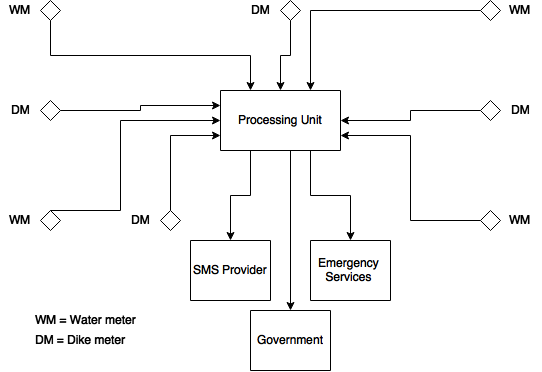
\includegraphics[width=90mm]{images/architecturalVision.png}
\caption{Schematic overview of the flood monitoring system}
\label{fig:architectural-vision}
\end{figure}

The smart flood monitoring system consists of multiple parts. First of all there is the monitoring part. This part monitors the current state of the environment. To achieve this, we need a lot of data. This data is obtained by sensors and weather data. We use sensors to get the current water level of waterways. We also measure the density and structure of dikes. The data that is obtained through all sensors will be automatically processed. The processed information represents a risk level for the area in which the system is deployed.

In case of an imminent flood a warning will be issued to the government and the citizens who live in the threatened area. We do this by issuing a warning to the government. In their turn the government uses their infrastructure to warn the citizens. In the Netherlands this infrastructure consists of a siren system and an SMS-system. Besides this people can also apply for our service. People who are subscribed to this service will receive a text message with more information about the (imminent) flood. 

In case of a real flood the citizens who subscribed to our service will receive a MMS message with a route to a safe area. These MMS messages contain generic routes to get to a safe area. This means that when a flood happens, the same map is send to different users.
%http://www.waterforum.net/Artikel/PrintArtikel.aspx?ID=9132
